Nei diagrammi di sequenza viene illustrata l'interazione tra il \gls{database} e i controller che recuperano i parametri, richiesti dai services del front-end, attraverso l'\gls{ORM} Eloquent fornito da \gls{Laravel}. Le associazioni tra richieste e controller sono mappate nel file \textit{routes.php}. Un controller termina la propria esecuzione restituendo al service del front-end un oggetto JSON che contiene:
\begin{itemize}
	\item i parametri corretti se la richiesta va a buon fine ed il metodo preveda il ritorno di essi;
	\item un messaggio di successo nel caso il metodo non preveda il ritorno di alcun paramento(es. salvataggio sul \gls{database});
	\item un messaggio di errore nel caso la richiesta non vada a buon fine.
\end{itemize}

\subsubsection{Richieste REST}
Si mostrano i diagrammi di sequenza di alcune chiamate REST che effettua il sistema per meglio specificarne il funzionamento.

\newpage

\textbf{GET user/:username/project}
	\begin{figure}[h]
		\centering
		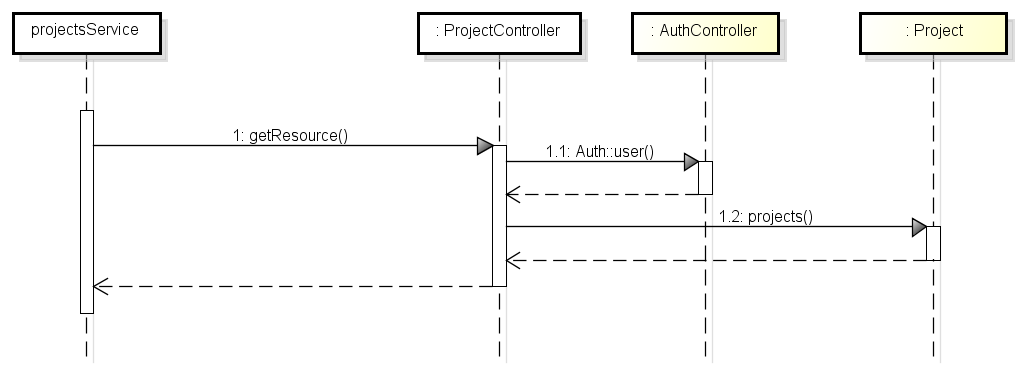
\includegraphics[width=0.7\linewidth]{img/GET_projects}
		\caption[GET user/:username/project]{GET user/:username/project}
		\label{fig:GET user/:username/project}
	\end{figure}

\textbf{POST user/:username/project}
	\begin{figure}[h]
		\centering
		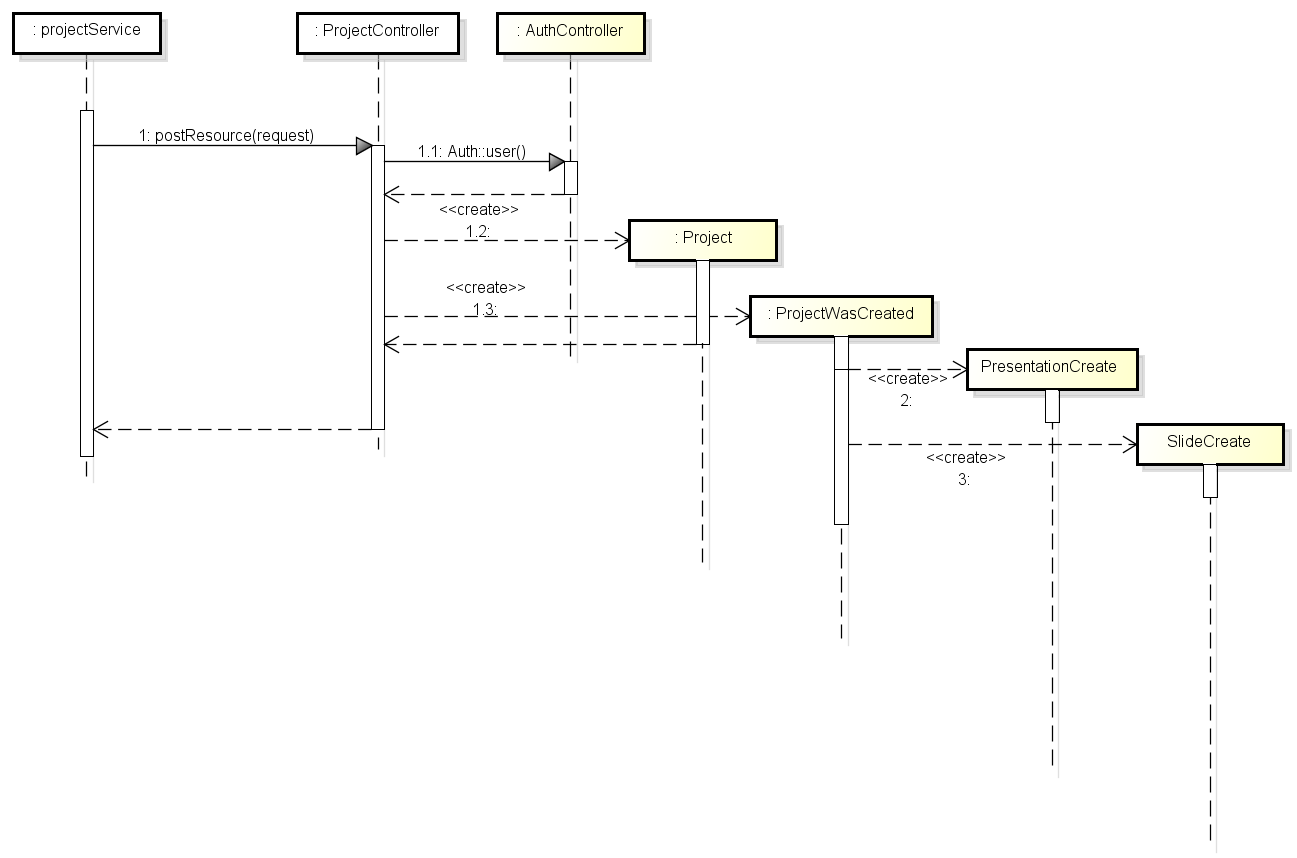
\includegraphics[width=0.6\linewidth]{img/POST_project}
		\caption[POST user/:username/project]{POST user/:username/project}
		\label{fig:POST user/:username/project}
	\end{figure}

\newpage

\textbf{PUT user/:username/project/:projectID}
	\begin{figure}[h]
		\centering
		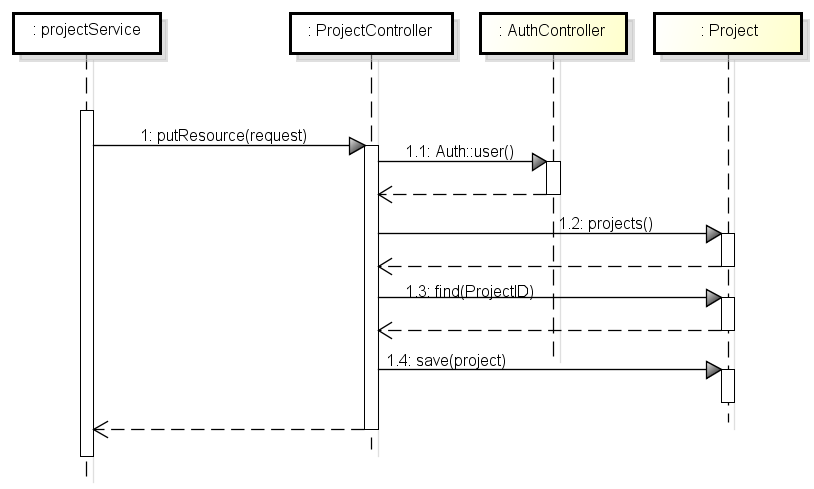
\includegraphics[width=0.6\linewidth]{img/PUT_project}
		\caption[PUT user/:username/project/:projectID]{PUT user/:username/project/:projectID}
		\label{fig:PUT user/:username/project/projectID}
	\end{figure}

\textbf{DELETE user/:username/project/projectID}
	\begin{figure}[h]
		\centering
		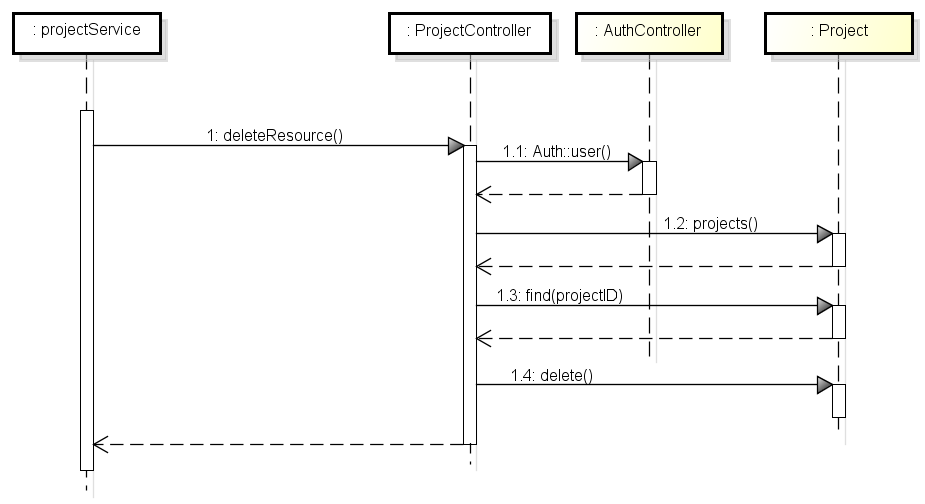
\includegraphics[width=0.6\linewidth]{img/DELETE_project}
		\caption[DELETE user/:username/project/:projectID]{DELETE user/:username/project/:projectID}
		\label{fig:DELETE user/:username/project/:projectID}
	\end{figure}